% vim: set spelllang=fr foldmethod=marker:
\section{Détection des attaques de déni de service}
\label{sa:sec:detection}
%===============================================================================
    \subsection{Usage des \cns}

À côté des nœuds «~normaux~» et des \chs, un troisième rôle va être attribué à certains capteurs, directement en lien avec la détection des attaques de type «~déni de service~».
Certains capteurs se voient ainsi confier le rôle de «~nœuds de contrôle~», ou \cns (introduits dans~\cite{LC08}), et sont chargés de surveiller le trafic entrant et sortant des \chs.

Si un \cn constate qu'un capteur envoie, au cours d'une unité de temps, plus de données à leur \CH qu'une valeur de seuil déterminée $S_{debit}$, il retient que le nœud a eu un comportement anormal (il y a eu un écart important à la moyenne de la quantité de données envoyées par unité de temps).
Lorsque ce nœud réalise un certains nombres d'écarts, \cad lorsque le nombre de comportement anormaux détectés par un \cn dépasse une valeur de seuil $S_{ecarts}$, le ou les nœuds de contrôle qui ont repéré ces écarts considèrent alors le capteur comme compromis.
Chaque \cn ayant détecté un nœud compromis envoie un message d'avertissement à son \ch.
Ici encore, un seuil $S_{alertes}$ est fixé pour le nombre minimum d'alertes qu'un \CH doit recevoir avant de considérer un nœud comme malveillant, et ce afin d'éviter qu'un nœud compromis se faisant passer pour un \cn ne déclare tous ses voisins comme compromis.
Plusieurs \cns distincts doivent donc détecter les écarts d'un nœud pour que celui-ci soit effectivement considéré comme compromis par le \ch.
Les messages en provenance des nœuds considérés malveillants par le \ch sont alors ignorés.

Les \cns comparent également la taille des trafics entrant et sortant du \ch.
En cas d'écart importants (en tenant compte des éventuels facteurs de compression des données et des messages ignorés des nœuds considérés compromis), ils peuvent être amenés à penser que le \ch est lui-même malveillant.
Dans ce cas, l'élection d'un nouveau \CH dans le cluster est déclenchée.

%===============================================================================
    \subsection{Objectifs à atteindre}

Le but de la solution proposée est de fournir un moyen efficace de lutter contre un nœud qui tenterait de corrompre les résultats envoyés à la station de base, ou bien de saturer les capacités de communication du réseau, en envoyant un flux de données plus important que les nœuds «~honnêtes~».
L'efficacité de cette méthode peut être mesurée sur deux aspects:
\begin{itemize}
    \item le taux de détection des nœuds compromis dans le réseau;
    \item la durée de vie du réseau.
\end{itemize}
Le second point peut être exprimé de plusieurs façons.
Par exemple, il est souvent défini comme la durée écoulée entre le déploiement du réseau et l'instant où le premier capteur à manquer d'énergie s'éteint.
Nous utiliserons nous aussi cette définition, qui implique que pour obtenir une grande durée de vie, la consommation en énergie du réseau doit être équitablement répartie entre un aussi grand nombre de nœuds que possible.

Pour obtenir une méthode efficace sur les deux points évoqués, nous proposons dès lors de mettre en place deux mécanismes: une partition hiérarchique des nœuds du réseau d'une part, et une élection dynamique des \cns d'autre part.

%===============================================================================
    \subsection{Partition hiérarchique du réseau}

Le fait de clusteriser le réseau de capteurs tel que présenté en \ssref{st:subsec:partition} permet de limiter la consommation en énergie de la plupart des nœuds du réseau, puisque seuls les \chs se retrouvent à effectuer des émissions sur des distances plus longues que le rayon d'un cluster.
La partition hiérarchique permet d'obtenir une gestion encore plus efficace des clusters, puisqu'elle introduit plus de granularité.
Nous proposons, pour notre solution (et pour nos tests, voir \sref{sa:sec:resultats}), une hiérarchie à deux degrés: nous avons clusterisé notre réseau en utilisant $k$-\leach, en fixant $k=2$ (voir figure~\ref{sa:fig:network}).
\begin{figure}[ht]
    \centering
    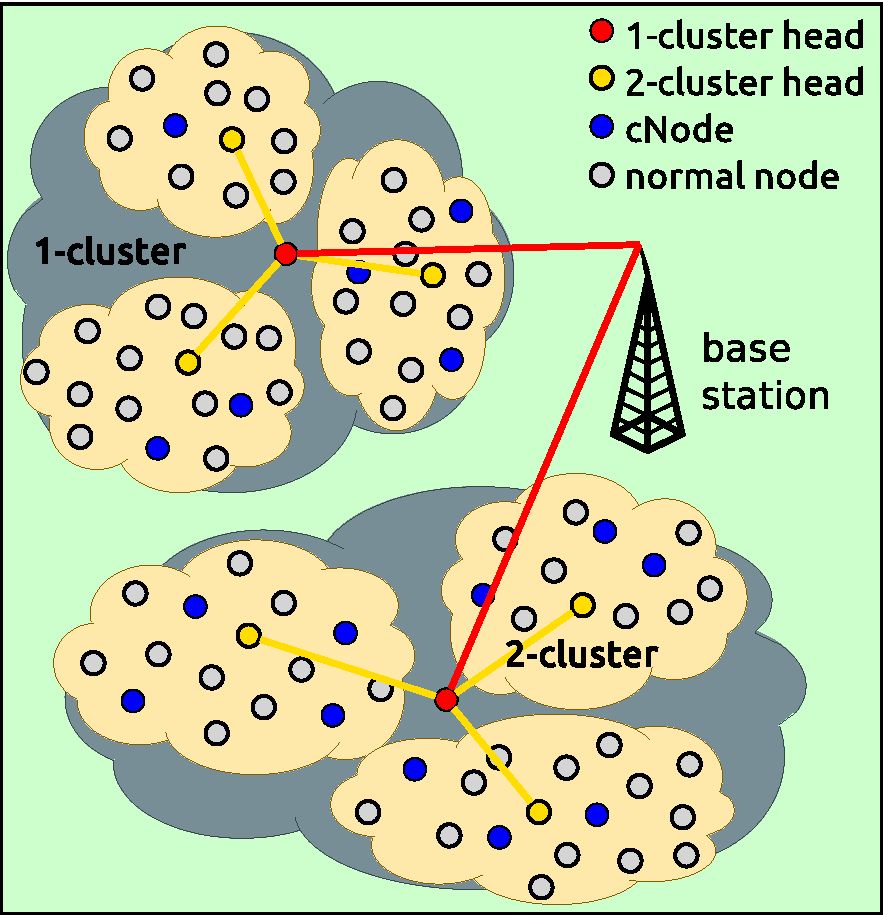
\includegraphics[width=.7\linewidth]{\chapterfig/network.pdf}
    \caption{Schéma du réseau avec deux niveaux de partition}\label{sa:fig:network}
\end{figure}
Ceci permet, à notre sens:
\begin{itemize}
    \item d'économiser davantage d'énergie par rapport à l'usage de \leach dans sa version simple;
    \item d'obtenir, en choisissant des \cns dans chacun des $2$-clusters, une meilleure couverture du réseau par les \cns, et de maximiser ainsi la probabilité de détection des nœuds compromis dans le réseau.
\end{itemize}
En pratique, $k$ doit être adapté en fonction du nombre de capteurs dans le réseau, de sa superficie, de la puissance et de la consommation énergétique des nœuds, mais nous n'avons pas de recommandations numériques plus poussées à présenter pour le moment.

%===============================================================================
    \subsection{Élection dynamique des \cns}

La partition du réseau permet de limiter aux seuls \chs les efforts énergétiques dus aux transmissions longues.
L'inconvénient est que, justement, ces \CH vont épuiser leur batterie beaucoup plus rapidement que s'ils étaient restés des nœuds ordinaires, tirant ainsi le réseau vers une fin de vie précoce.
Heureusement, les nœuds ne sont pas désignés \CH «~à vie~».
\leach renouvelle périodiquement la partition du réseau, choisissant à chaque itération de nouveaux \chs.

Mais s'ils n'émettent pas sur de longues distances, les \cns se retrouvent eux aussi à consommer plus d'énergie que les nœuds normaux, puisqu'il doivent sans cesse rester en écoute des transmissions qui les entourent, et analyser le débit de chacun de leurs voisins.
Pour répartir cette nouvelle charge, qui touche davantage de nœuds, nous proposons d'élire également les \cns de façon dynamique, sur une période plus courte que celle correspondant à la clusterisation du réseau.
Cette solution améliore aussi la sécurité du réseau: si un attaquant cherche à compromettre tous les \cns du cluster, pour pouvoir poursuivre son attaque discrètement, le renouvellement dynamique apporte une parade efficace à l'attaque.

À chaque étape, la sélection des \cns est censée être aléatoire.
L'aléatoire est une notion délicate en informatique; nous nous contenterons plutôt d'un algorithme capable de générer des nombres dits «~pseudo-aléatoires~».
Une façon de procéder, par exemple, est de recourir à un algorithme capable de générer une suite de nombre d'apparence aléatoire, utilisés pour déterminer quels seront les \cns pour la période à venir~\cite{GMT12}.
Cet algorithme se doit de respecter les points suivants:
\begin{itemize}
    \item il doit nécessiter peu de calculs;
    \item sa période doit être grande;
    \item les valeurs générées doivent être indépendantes et distribuées uniformément.
\end{itemize}
Nous nous sommes tournés vers un type connu de générateurs, les \textit{Multiplicative Linear-Congruential Generators} (ou MLCG), possédant une grande période~\cite{RJ91}.
Plus précisément, le générateur retenu est de type $x_n = a\cdot x_{n-1}\bmod m$, où:
\begin{itemize}
    \item le nombre pseudo-aléatoire $x_n$ est généré en fonction de son prédécesseur $x_{n-1}$;
    \item $m$ est de la forme $2^k$, ce qui facilite le calcul de $\bmod m$ (troncature à droite du résultat sur $k$ bits);
    \item $a$ doit être de la forme $8\cdot i\pm3$ (avec $i$ un entier positif) pour que le générateur ait la période maximale, égale à $2^{k-2}$;
    \item $x_0$ (la «~graine~», ou \textit{seed} en anglais) doit être un entier impair (toujours pour avoir la meilleure période).
\end{itemize}
La méthode de Schrage permet de reformuler le générateur sous une forme qui prévient tout problème de débordement\footnote{Un débordement désigne le dépassement, au cours des calculs, de la valeur d'entier maximale gérée par le système, qui se traduit par des erreurs de calcul.} lors de l'implémentation~\cite{RJ91}.
Le générateur est alors écrit sous la forme suivante: $a\cdot x\bmod m=g(x)+m\cdot h(x)$, avec:
\[\left\{
    \begin{aligned}
        g(x) & =a\cdot(x\bmod q)-r\cdot(x\mbox{~div~}q)\\
        h(x) & =(x\mbox{~div~}q)-(a\cdot x)\mbox{~div~}m\\
        q    & =m\mbox{~div~}a\\
        r    & =m\bmod a
    \end{aligned}
\right.\]
Voici finalement un exemple de générateur (il s'agit de celui qui a été implémenté pour réaliser les tests présentés en \sref{sa:sec:resultats}):
\[x_n=11\cdot x_{n-1}\bmod2^{16}\]
Sa période est égale à $2^{14}$.
Ce générateur peut alors être utiliser pour calculer des nombres pseudo-aléatoires allant de $0$ à $65535$ qui, ramenés sur le nombre attendu de \cns dans le cluster, permettent de déterminer quels vont être les nœuds élus pour la période en cours.
Il convient naturellement d'attribuer une graine différente à chaque nœud du réseau, afin d'éviter que tous les nœuds produisent la même suite de nombres pseudo-aléatoires.
Ceci peut être réalisé en initialisant l'algorithme avec une mesure physique ---~après tout, il s'agit de capteurs!~--- dont la valeur est ramenée à l'entier impair le plus proche.

Mais une question subsiste: quelle va-t-être l'entité chargée d'exécuter cet algorithme et de procéder à l'élection des \cns?
Trois méthodes différentes sont ici proposées: une auto-élection distribuée, une élection centralisée au niveau des \CH, ou alors une élection centralisée au niveau de la station de base.
%===============================================================================
    \subsection{Processus d'élection des \cns}

        \subsubsection{Auto-élection distribuée}
Une première solution consiste à réutiliser l'algorithme d'auto-désignation mis en œuvre par \leach, comme présenté sur la figure~\ref{sa:fig:elecself}.
\begin{figure}[ht]
    \centering
    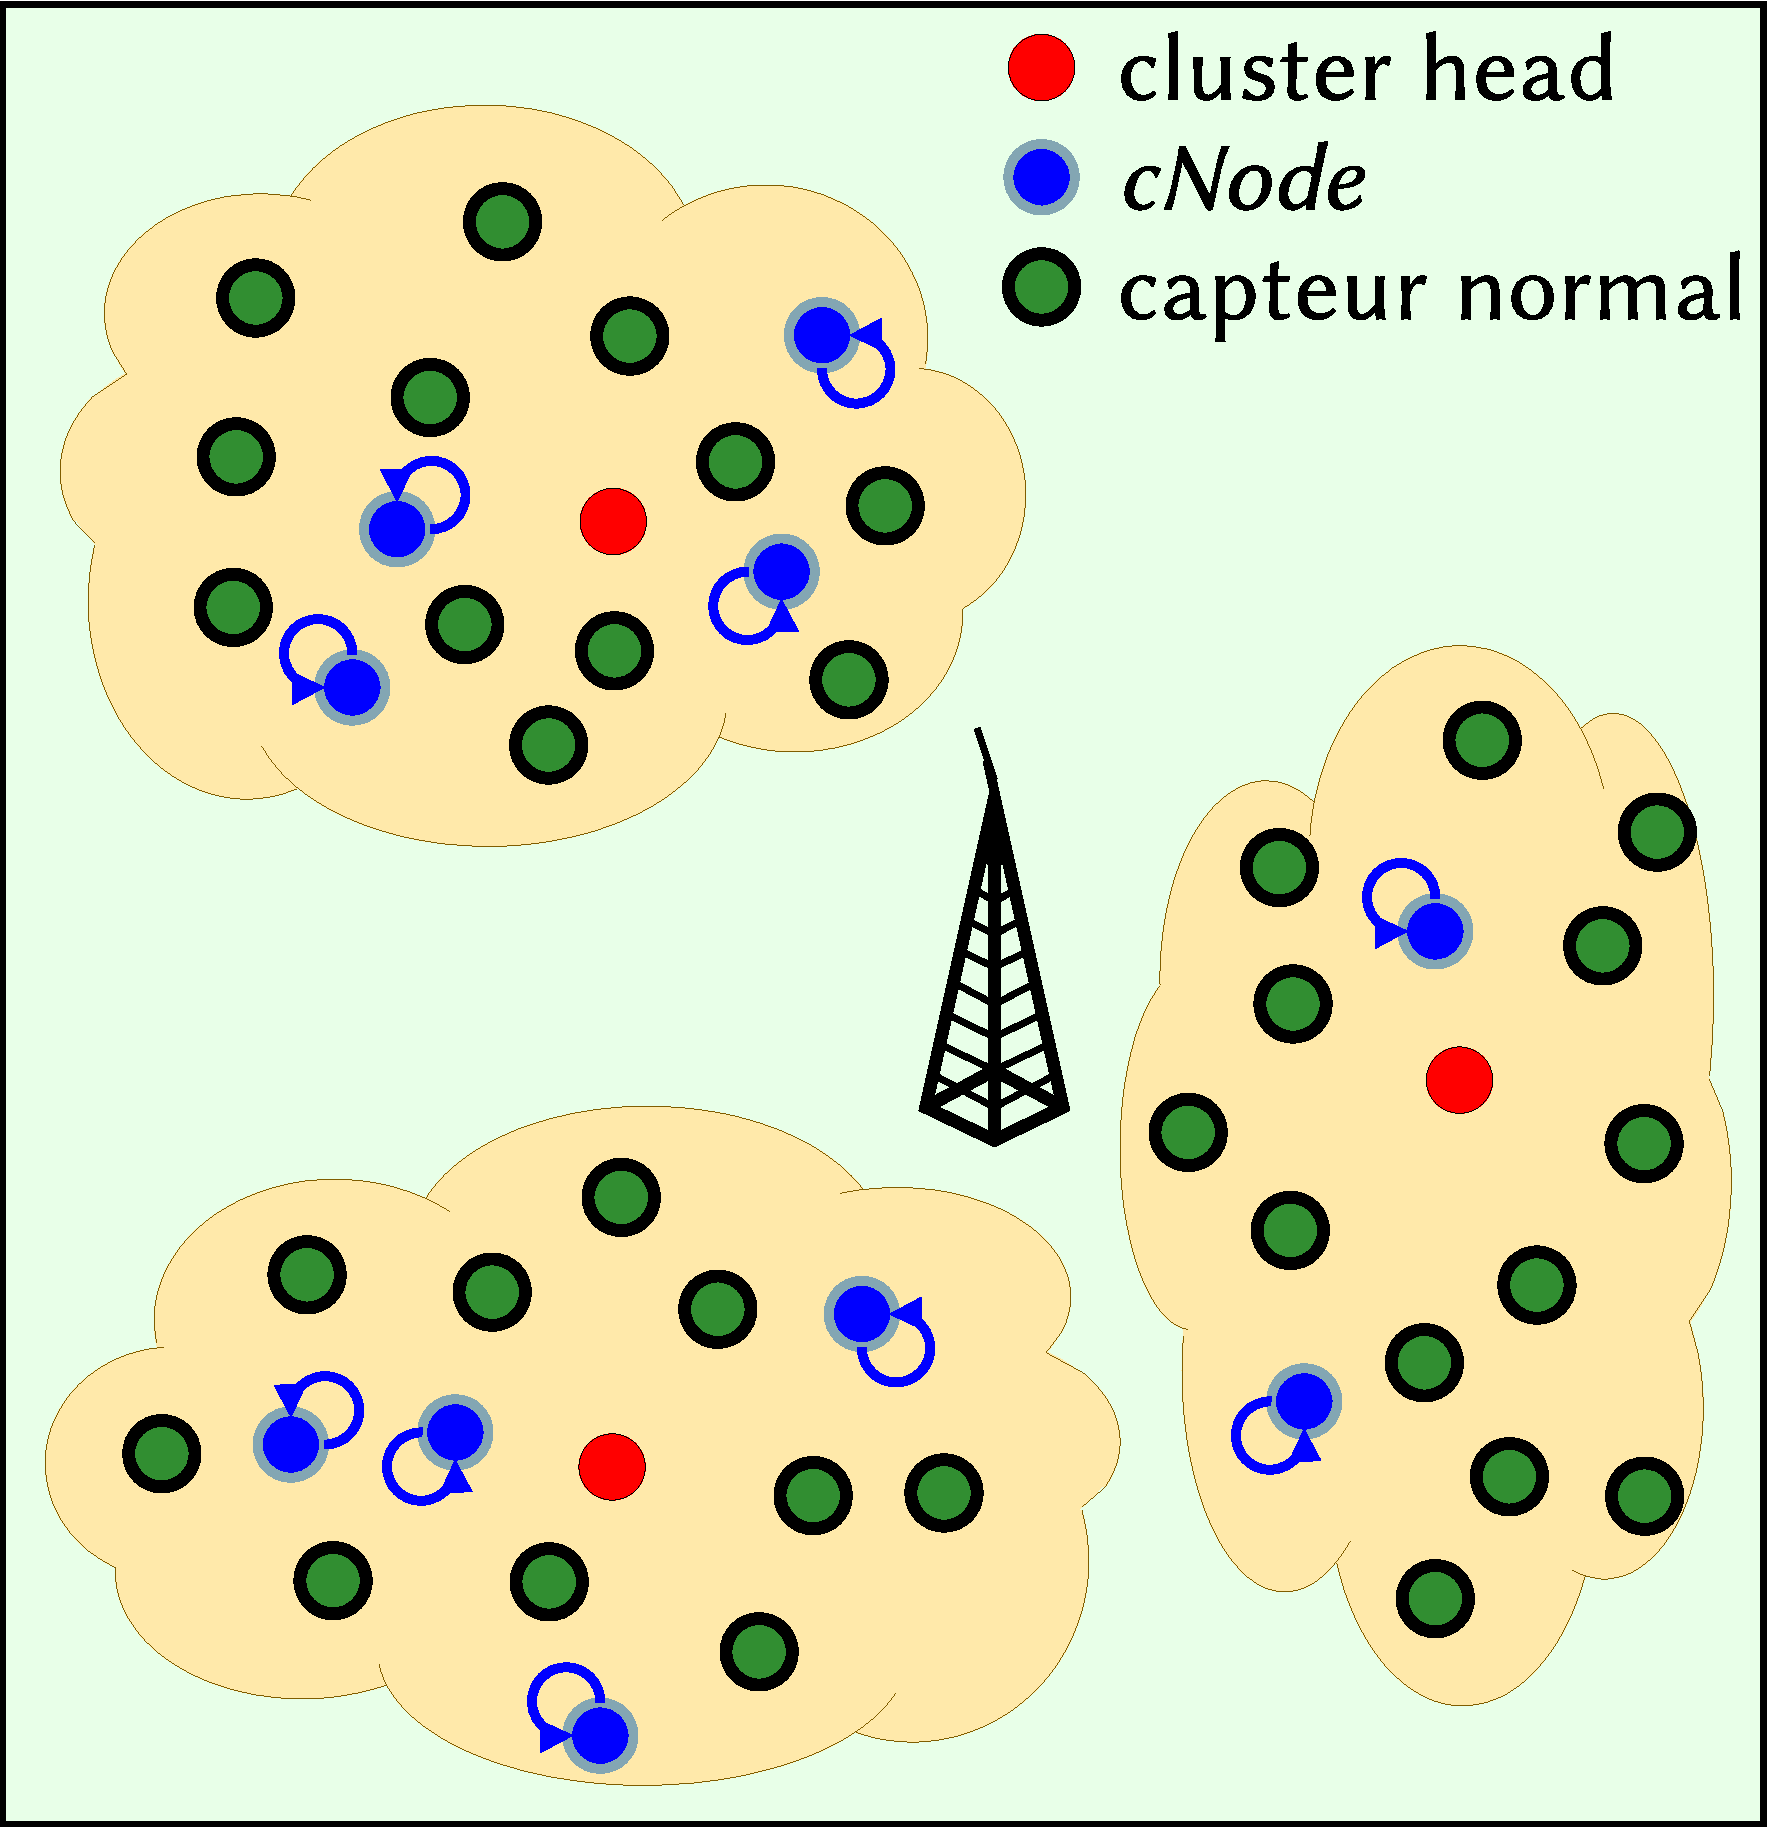
\includegraphics[width=.5\linewidth]{\chapterfig/elec_self.pdf}
    \caption{Auto-élection des \cns}\label{sa:fig:elecself}
\end{figure}
Chaque nœud non \CH choisit un nombre pseudo-aléatoire compris entre 0 et 1.
Si ce nombre est en-dessous du pourcentage de \cns désirés dans le réseau (et fixé au moment de l'implémentation par l'utilisateur), ce nœud devient un \cn.
Autrement, il reste un capteur normal.

Cette méthode présente deux inconvénients.
Tout d'abord, elle impose à chaque nœud de calculer un nombre pseudo-aléatoire --- calcul parfois coûteux ---, ce qui n'est pas nécessaire avec les deux autres méthodes.
Ensuite, chaque nœud choisit lui-même de se désigner (ou non) \cn, sans tenir compte de la décision de ses voisins.
Si bien que l'élection des \cns ne prend en compte à aucun moment la clusterisation du réseau.
Il est très peu probable que les \cns ainsi élus soient uniformément répartis entre les différents $2$-clusters du réseau.
Il est même possible que certains $2$-clusters se retrouvent totalement dépourvus de \cns (et se retrouvent ainsi dans l'incapacité de détecter une attaque).

Ce second point peut être contourné en menant une élection en deux étapes.
Dans un premier temps les nœuds choisissent d'endosser, ou non, le rôle de \cn; les \cns élus signalent alors leur statut au $2$-\CH auquel ils sont associés.
Au cours de la seconde étape, les $2$-\CH nomment des \cns supplémentaires dans leurs $2$-clusters respectifs si le nombre de signalements reçu au regard du nombre de nœuds dans les $2$-clusters est en-dessous d'un pourcentage minimal.

        \subsubsection{Élection centralisée au niveau des \chs}
        La seconde méthode proposée consiste à décharger les nœuds du processus d'auto-désignation, pour le remplacer par une nomination autoritaire réalisée par les $2$-\chs (voir figure~\ref{sa:fig:elecch}).
\begin{figure}[ht]
    \centering
    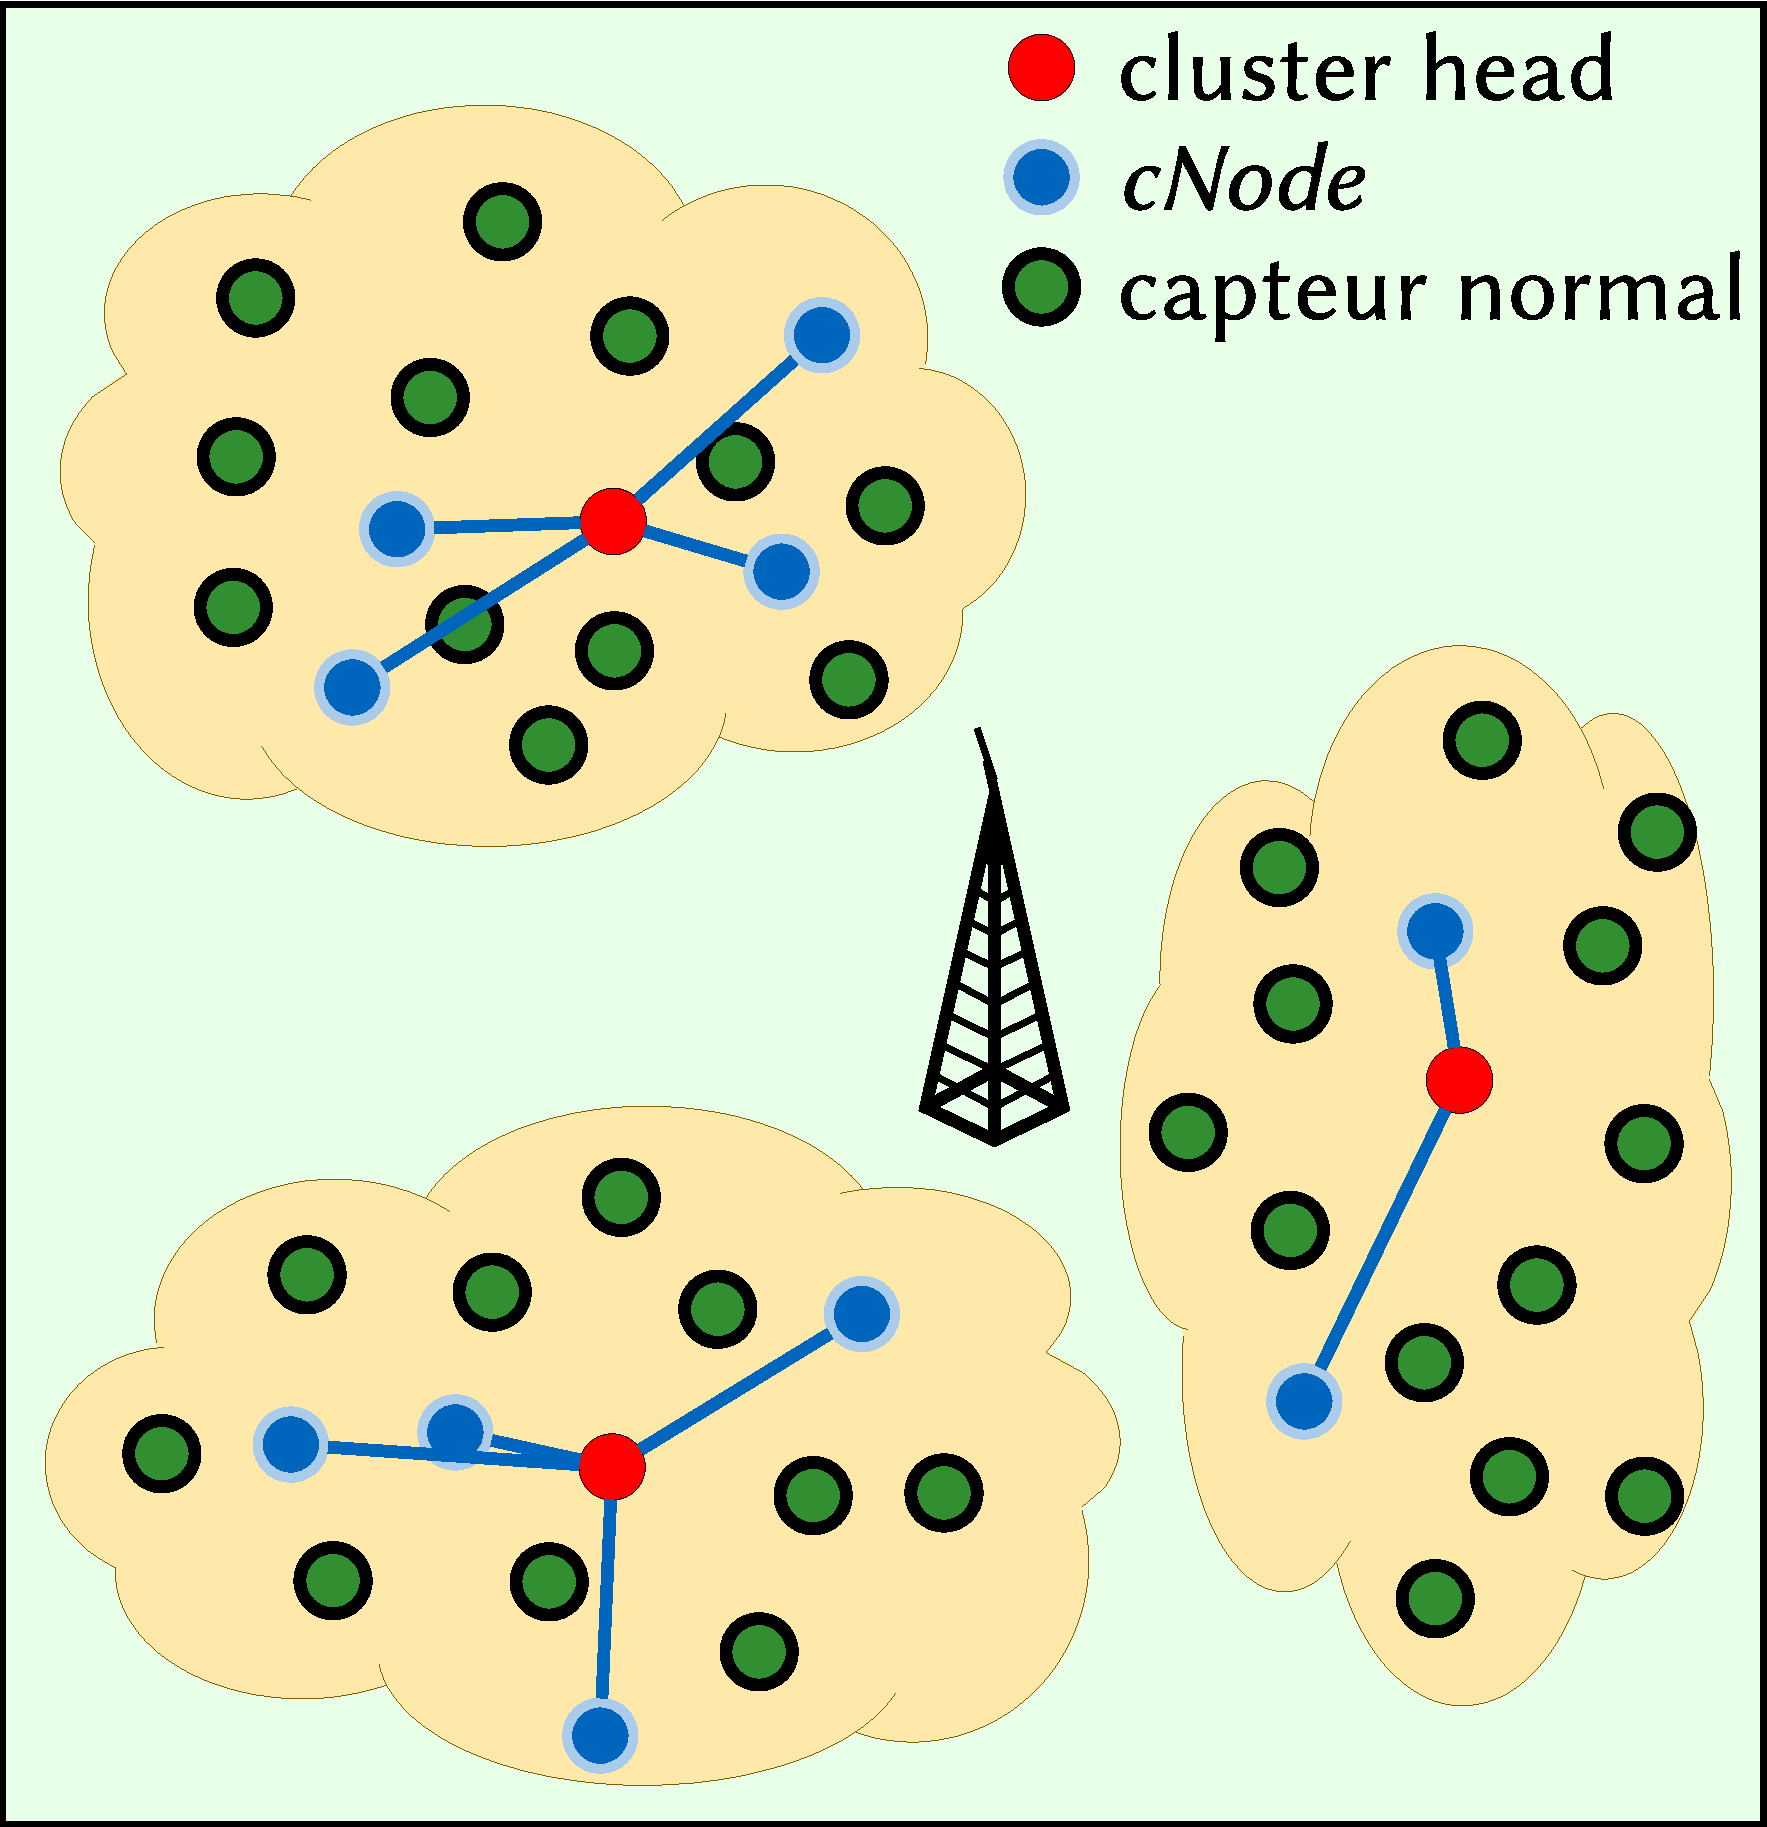
\includegraphics[width=.5\linewidth]{\chapterfig/elec_ch.pdf}
    \caption{Élection des \cns réalisée par les \ch}\label{sa:fig:elecch}
\end{figure}
Chaque \CH désigne alors un nombre de \cns correspondant au pourcentage indiqué par l'utilisateur.
Par exemple, si l'on souhaite obtenir dix pour cent de \cns, et qu'un $2$-cluster comporte cent capteurs, le \CH de ce cluster va produire dix nombre pseudo-aléatoires distincts qui seront associés aux identifiants de dix nœuds du cluster.
Le \CH envoie alors un message à chacun de ces dix nœuds pour leur ordonner de remplir le rôle de \cn sur la période en cours.

Cette méthode est plus efficace en terme de calculs puisque seul les $2$-\CH ont à appliquer un algorithme de calcul de nombres pseudo-aléatoires.
Cependant, elle présente un autre désavantage: si l'un de ces \CH est compromis par un attaquant, il ne déclarera sans doute aucun \cn susceptible de le détecter, laissant ainsi tout son cluster à la merci d'autres attaques.
Comme l'algorithme \leach désigne à tour de rôle chaque capteur, sur un cycle complet, pour accomplir le rôle de \CH, tout nœud compromis deviendra logiquement \CH à un moment ou l'autre.
Le problème du \CH ne désignant aucun \cn peut donc légitimement se poser pour n'importe quel nœud compromis du réseau.
Qui plus est, il faut garder à l'esprit que rien n'empêche un nœud compromis de se déclarer \ch à chaque ronde de l'algorithme \leach.

Cette méthode est néanmoins celle qui est implémentée dans les travaux de la référence~\cite{GMT12}, et que nous reprenons pour nos tests (dont les résultats sont disponibles en \sref{sa:sec:resultats}).

        \subsubsection{Élection centralisée au niveau de la station de base}
L'élection centralisée peut également être effectuée au niveau de la station de base (\BS), comme représenté sur la figure~\ref{sa:fig:elecbs}.
\begin{figure}[ht]
    \centering
    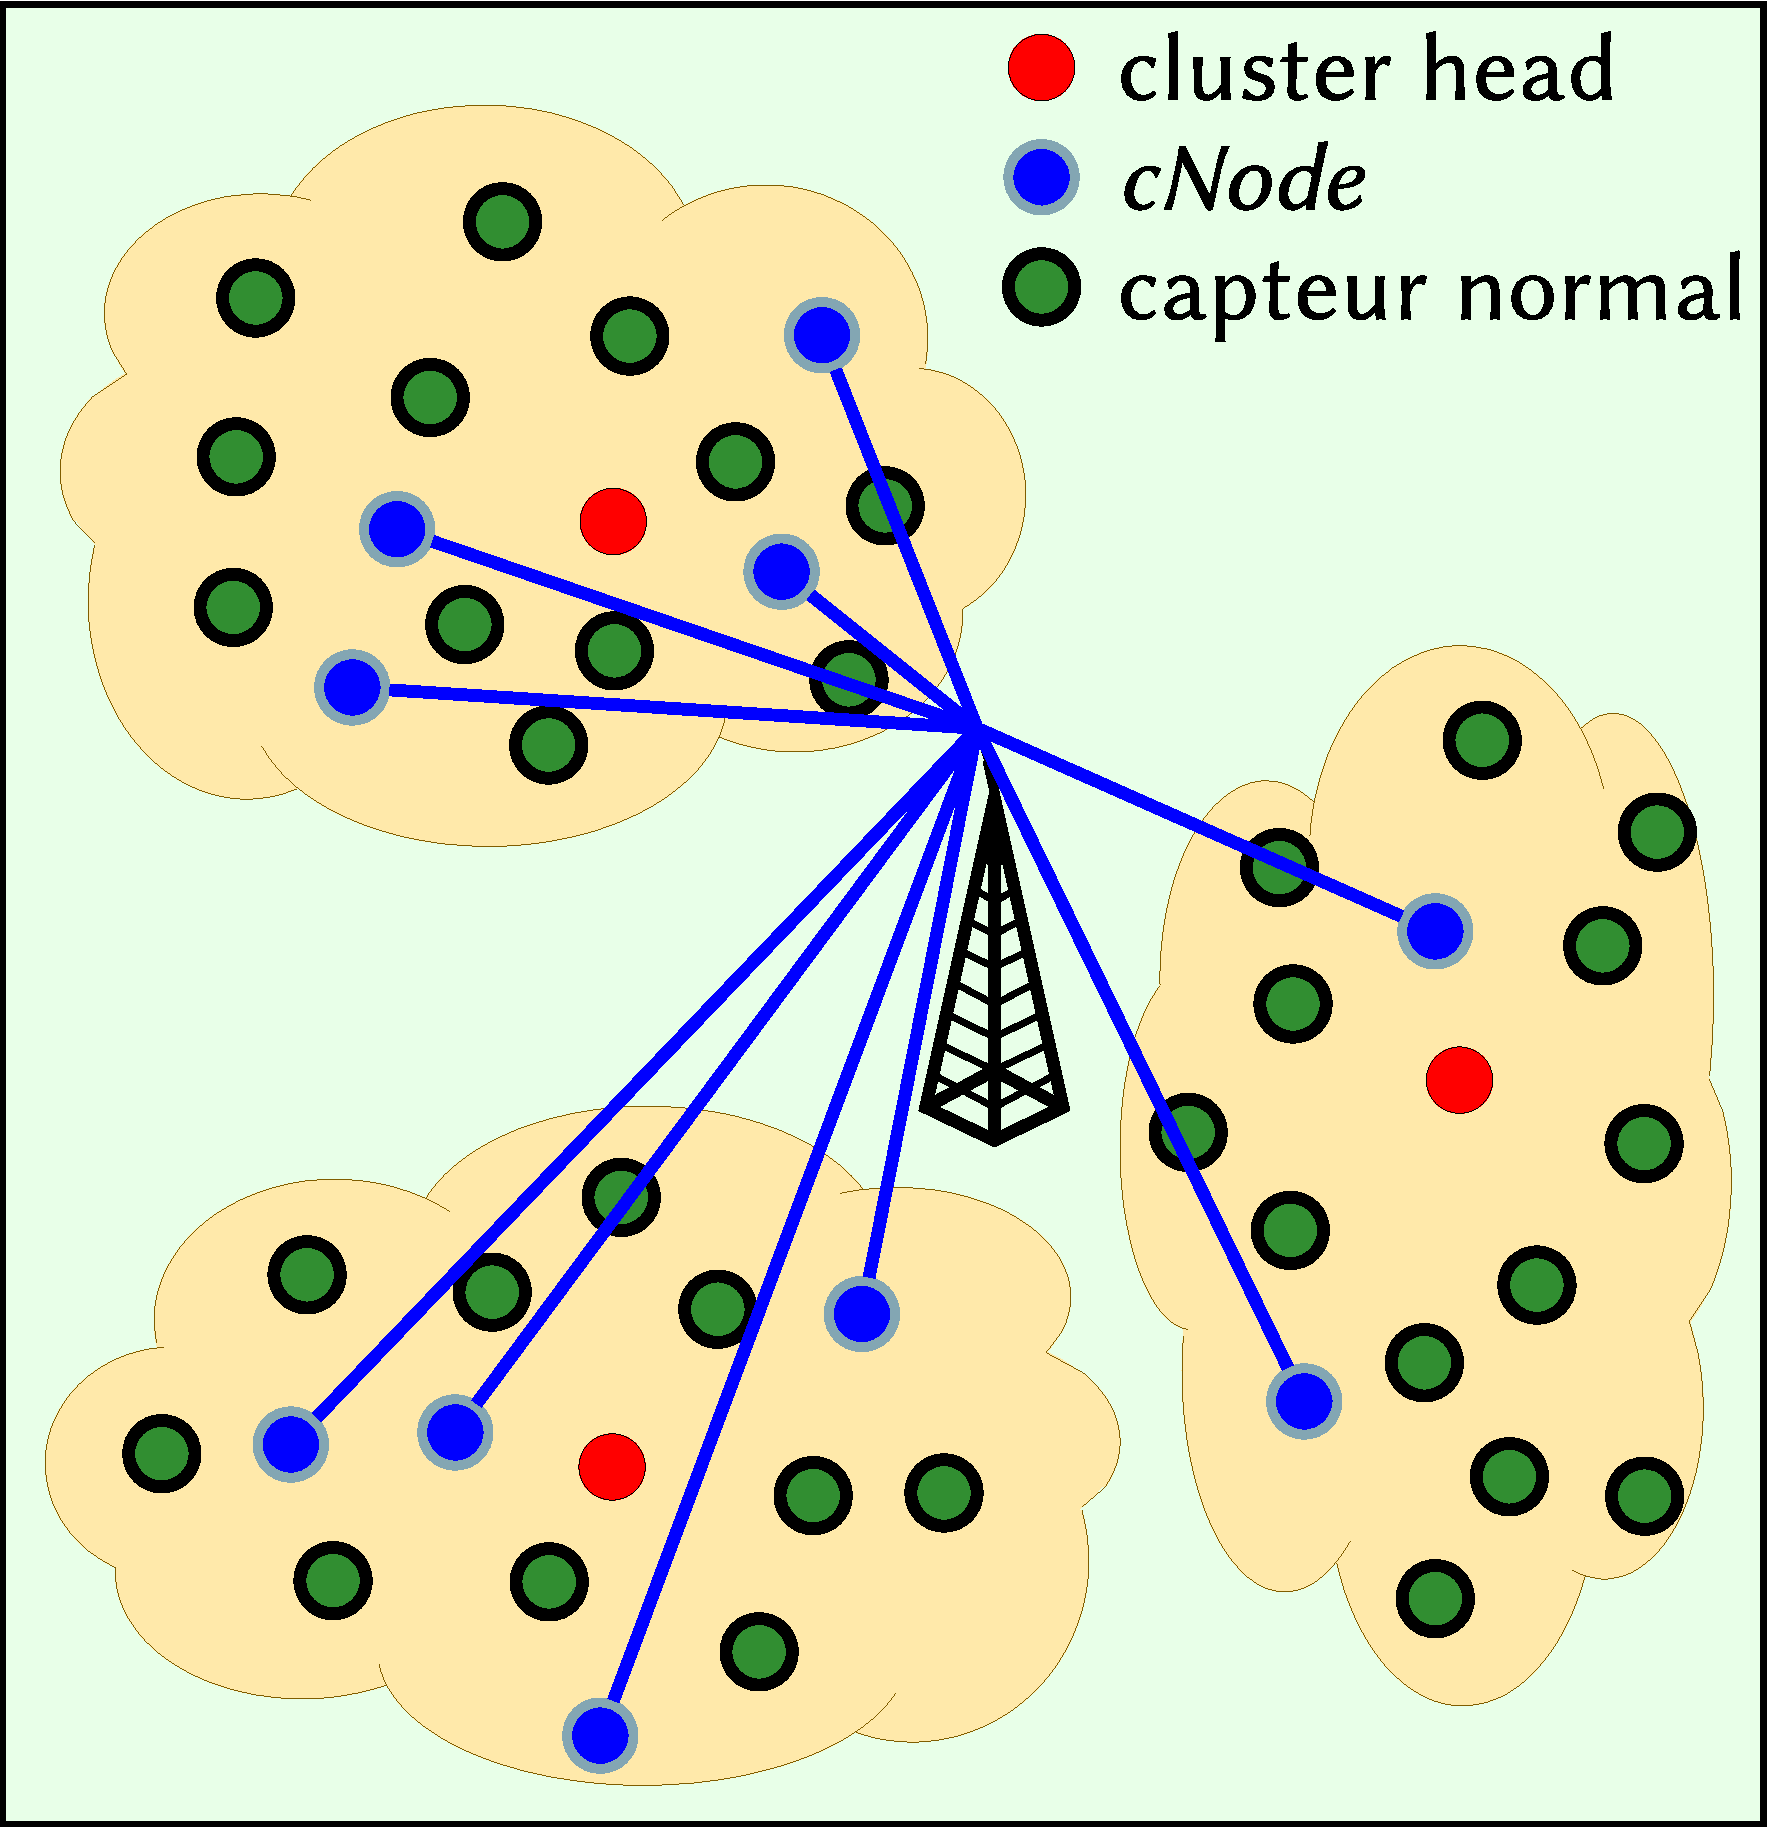
\includegraphics[width=.5\linewidth]{\chapterfig/elec_bs.pdf}
    \caption{Élection des \cns réalisée par la station de base}\label{sa:fig:elecbs}
\end{figure}
Les $2$-\CH du réseau font alors remonter à la \BS la liste des nœuds de leurs $2$-clusters respectifs, et la \BS retourne une liste de \cns pour chacun d'entre eux.
Les capacités (en mémoire, calcul, énergie) de la station de base étant considérées comme illimitées, cette méthode a pour avantage de déporter toutes les tâches coûteuses dans un environnement «~sans contraintes~».
Le calcul des nombres pseudo-aléatoires par la station de base ne lui coûte, pour ainsi dire, rien.

En revanche cette méthode n'offre pas une meilleure fiabilité que la précédente.
Si un nœud compromis se déclare en temps que \CH, il risque fortement d'annoncer à la \BS que son cluster est vide (il enverrait une liste vide en lieu et place de la liste des capteurs qui sont réellement présents dans son cluster).
Dans ce cas, la station de base ne déclarera aucun \cn dans le cluster attaqué, et le \CH compromis ne sera pas détecté.
Pour parer à cette éventualité, la station de base pourrait agir autrement lorsqu'elle reçoit une liste de capteurs vide.
Plus spécifiquement, elle devrait considérer que les nœuds dont elle n'a pas eu de nouvelles \via les listes des \CH ne sont peut-être pas simplement morts, mais escamotés par un \ch corrompu.
Ces nœuds disparus devraient donc être considérés comme potentiellement éligibles, de sorte que certains d'entre eux au moins soient déclarés \cns.

L'inconvénient majeur de cette méthode est le fait que la nature distribuée de l'élection (avec tous les avantages qu'apporte un algorithme distribué) est complètement
perdue.

Les avantages et inconvénients de chacune de ces trois méthodes présentées sont résumés dans la \tabref{sa:table:elec}.
\begin{table}[ht]
    \caption{Avantages et inconvénients de chaque méthode}\label{sa:table:elec}
    \medskip
    \begin{small}
        \begin{tabular}{m{.2\textwidth} m{.35\textwidth} m{.35\textwidth}}
            \toprule
            \centering \textsc{Méthode} & \centering \textsc{Avantages} & \centering \textsc{Inconvénients} \tabularnewline
            \midrule
            \centering Auto-élection des \cns (selon le modèle de \leach)    & %
                        \textbullet~Très simple à mettre en œuvre\newline%
                        \textbullet~Pas d'envoi de paquets à travers le réseau pour désigner les \cns%
                        & %
                        \textbullet~Chaque nœud doit calculer un nombre pseudo-aléatoire\newline%
                        \textbullet~Ne tient pas compte de la topologie du réseau\tabularnewline
            \midrule
            \centering Élection des \cns par les \ch                        & %
                        \textbullet~Seuls les \CH calculent les nombres pseudo-aléatoires%
                        & %
                        \textbullet~Si le \CH est compromis, il ne désigne aucun \cn (un nœud compromis peut se déclarer \CH à chaque ronde de \leach)\tabularnewline
            \midrule
            \centering Élection des \cns par la station de base                & %
                        \textbullet~Aucun calcul réalisé par les nœuds\newline%
                        \textbullet~Distribution spatiale idéale des \cns%
                        & %
                        \textbullet~Si le \CH est compromis, il déclare un cluster vide\newline%
                        \textbullet~Perte de l'aspect centralisé de l'algorithme\tabularnewline
            \bottomrule
        \end{tabular}
    \end{small}
\end{table}
